% TO-DO:

\input{../YKY-preamble.tex}

\usepackage{color}
\usepackage{mathtools}
\usepackage{hyperref}

\usepackage[backend=biber,style=numeric]{biblatex}
\bibliography{../AGI-book}
% \renewcommand*{\bibfont}{\footnotesize}

\usepackage{graphicx} % Allows including images
\usepackage{tikz-cd}
% \usepackage{tikz}
\usepackage[export]{adjustbox}% http://ctan.org/pkg/adjustbox
\usepackage{verbatim} % for comments
% \usepackage{tikz-cd}  % commutative diagrams
% \newcommand{\tikzmark}[1]{\tikz[overlay,remember picture] \node (#1) {};}
% \usepackage{booktabs} % Allows the use of \toprule, \midrule and \bottomrule in tables
% \usepackage{amssymb}  % \leftrightharpoons
% \usepackage{wasysym} % frownie face
% \usepackage{newtxtext,newtxmath}	% Times New Roman font
% \usepackage{sansmath}

\newcommand{\underdash}[1]{%
	\tikz[baseline=(toUnderline.base)]{
		\node[inner sep=1pt,outer sep=10pt] (toUnderline) {#1};
		\draw[dashed] ([yshift=-0pt]toUnderline.south west) -- ([yshift=-0pt]toUnderline.south east);
	}%
}%

\DeclareSymbolFont{symbolsC}{U}{txsyc}{m}{n}
\DeclareMathSymbol{\strictif}{\mathrel}{symbolsC}{74}

\newcommand{\emp}[1]{{\color{violet}\textbf{#1}}}
\newcommand*\confoundFace{$\vcenter{\hbox{\includegraphics[scale=0.2]{../confounded-face.jpg}}}$}

\begin{document}

\title{\cc{\bfseries\color{blue}{\Huge《AGI 逻辑导论》}}
{{\Huge《AGI logic tutorial》} }}
\author{YKY} % Your name
%\institute[] % Your institution as it will appear on the bottom of every slide, may be shorthand to save space
%{
%Independent researcher, Hong Kong \\ % Your institution for the title page
%\medskip
%\textit{generic.intelligence@gmail.com} % Your email address
%}
\date{\today} % Date, can be changed to a custom date

\maketitle

\section*{Summary}
\begin{itemize}
	\item 描述一种可以完整地解决 AGI 的逻辑
\end{itemize}

\tableofcontents
% \vspace*{0.5cm}
% 多谢 支持 \smiley


\section{Background}

An AI is essentially a dynamical system that constantly updates its ``state'' $\vect{x}$:
\begin{equation}
\dot{\vect{x}} = \vect{F}(\vect{x})
\end{equation}

Part of the state $\vect{x}$ contains \emp{sensory input} and \emp{action output} that allow the AI to interact with the external environment.



\section{Structure of logic}

The central tenet of my theory is that the state $\vect{x}$ of the AI system is consisted of \emp{logic propositions} and that $\vect{F}$ plays the role of the \emp{logic consequence} operator $\vdash$:
\begin{equation}
\begin{tikzcd}
\boxed{\mbox{propositions}}
\arrow[r, tail, no head, "\vect{F}"]
& \boxed{\mbox{propositions}}
\end{tikzcd}
\end{equation}

So our goal now is to elucidate the structure of $\vdash$.  Currently the most elegant formulation is given by \emp{categorical logic} or \emp{topos theory}.

我发觉 我是一个擅长於 ``synthesize'' 的人,意思是我会看很多书,然后将各种 分散的 ideas 融合成一个 内部协调 的理论(当中大部分 ideas 不是我原创的)。

在接下来的篇幅,我会勾划一个 对於 AGI 来说是完整的 逻辑理论,而这理论 最中心的思想 是 Curry-Howard isomorphism....

\section{Curry-Howard correspondence}

Curry-Howard isomorphism 是一个很深刻的思想,如果不小心的话 甚至会觉得它讲了等於没讲。 

%The Curry-Howard correspondence is a deep connection between logic and computation (in the form of type theory).

它已经被发现了很多次,实际上它的发现者包括: Brouwer-Heyting-Kolmogorov-Sch\"{o}nfinkel-Curry-Meredith-Kleene-Feys-G\"{o}del-L\"{a}uchli-Kreisel-Tait-Lawvere-Howard-\mbox{de Bruijn}-Scott-Martin-L\"{o}f-Girard-Reynolds-Stenlund-Constable-Coquand-Huet-\-Lambek ....

Curry-Howard isomorphism 讲的是 \emp{逻辑} 与 \emp{计算} 之间的同构,但在 1990s Lambek 加上了 \emp{category theory},所以现在不少人会讲 Curry-Howard- Lambek.  事实上,逻辑-计算-范畴论 这个「三角关系」之间的相互作用非常丰富,人们认为是未来发展的思想泉源。 

简单来说: 当我们做 逻辑思考时,表面上有一种语法上 (syntax) 的形式,即 $A \Rightarrow B$:
\begin{equation}
\begin{aligned}
\boxed{\mbox{logic}} \quad \quad \underdash{$A \Rightarrow B$} & \\
\boxed{\mbox{program}} \quad \quad \square \stackrel{f}{\mapsto} \square \hspace{10pt} &
\end{aligned}
\end{equation}
而在这 语法「底下」,还有一个 \emp{运算},它可以看成是执行 \emp{证明} (proof) 的工作,它将 $A$ 的证明 map 到 $B$ 的证明 (为了避免符号累赘,我将这些 ``proof witness'' 都记作 $\square$,但它们每个是不同的).

从另一角度看,Curry-Howard isomorphism 可以看成是 某些 \emp{状态}(states,例如 $A$)和状态之间的 \emp{转换} (transitions,例如 $\stackrel{f}{\mapsto}$)之间的 \textbf{对偶}。 而这种 对偶 不断在 截然不同的范畴里出现:
\begin{equation}
\begin{tabular}{|c|c|c|c|c|}
	\hline 
	\textbf{logic} & \textbf{computation} & \textbf{category theory} & \textbf{physics} & \textbf{topology} \\ 
	\hline \hline
	proposition & type & object & system & manifold \\ 
	\hline 
	proof & term & morphism & process & cobordism \\ 
	\hline 
\end{tabular} 
\end{equation}
前两个就是 Curry-Howard,第三个 是 Lambek 加上去的,其馀的来自 John Baez \& M. Stay 的论文: \textit{Physics, Topology, Logic and Computation: a Rosetta stone} [2010].  例如在 physics 里面是 Hilbert space 和 operators 的对偶; 在 topology 里面,cobordism 的著名例子就是这个 ``pair of pants'':
\begin{equation}
\vcenter{\hbox{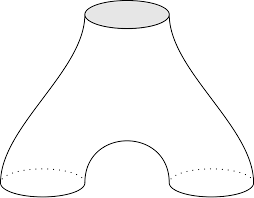
\includegraphics[scale=0.3]{pair-of-pants.png}}}
\end{equation}
In string theory,它表示上面的 strings 变成下面的 string 的「时间过程」。

\subsection{Type theory}

描述 \emp{program} 或 \emp{computation} 的语言叫 type theory.  例如在一般的 编程语言 里可以有这样的一句:
\begin{equation}
\begin{small}
\verb!define length(s: String): Integer = { .... }!
\end{small}
\end{equation}
意思是说 length() 是一个函数,输入 String,输出 Integer.

在数学里 我们描述 \emp{函数} 时会用:
\begin{equation}
f: A \rightarrow B
\end{equation}
这个表达式其实就是 type theory 的一般形式:
\begin{equation}
\overbrace{t}^{\mbox{term}} : \overbrace{T}^{\mbox{type}}
\end{equation}
而这个 notation $t:T$ 其实也可以写成 $t \in T$(但不正统而已)。 

换句话说,types 就是 \textbf{集合},terms 是集合中的 \textbf{元素}。 

更一般地,一个 type theory 的句子 可以包含 type \emp{context}:
\begin{equation}
\overbrace{x : A}^{\mbox{context}} \vdash \overbrace{f(x) : B}^{\mbox{type assignment}}
\end{equation}
意思就像在 program 的开头 ``declare'' 一些 变量 的类型,然后 program 就可以被 \emp{赋予} 后面的 类型。 

这个 $\vdash$ 的过程 称为 \emp{type assignment},而这就是 type theory 做的全部工作。 

\subsubsection{$\lambda$-calculus}

在一个 program 里,除了定义 类型,还需要定义 \emp{函数}。 这件工作是由 $\lambda$-calculus 负责。

$\lambda$-calculus 可以定义函数 而不需要提及它的「名字」。 例如,用数学式表达:
\begin{equation}
f(x) \triangleq x^2
\end{equation}
它的 $\lambda$-表达式就是:
\begin{equation}
f \triangleq \lambda x. \; x^2
\end{equation}
注意: 在 $\lambda$-表达式里,不需要提到 $f$ 的「名字」。

$\lambda$-calculus 是由 Alonso Church 发明,目的是研究数学上 \emp{substitution} 的性质。 Substitute 是每个中学生都懂得做的事,但要用数学表达出来却是出奇地麻烦。 

同时,Church 发现 $\lambda$-calculus 是一种「万有」的计算形式,和 \emp{Turing machines} 等效。 「AI 之父」John McCarthy 用 $\lambda$-calculus 发展出 \emp{Lisp} 语言,它是所有 functional programming language 的鼻祖。 

\subsubsection{Curry-Howard correspondence}

在 Curry-Howard 对应下,type $A$ 就是 逻辑命题 $A$,type $A$ 或 集合 $A$ 里面的 元素 是其 \textbf{证明} (proof, or proof witness)。

而,$A \Rightarrow B$ 也是 逻辑命题,它对应於 the function type $A \rightarrow B$,也可以写作 $B^A$,而这个 type 或 集合 里面的 元素 就是一些 函数 $f: A \rightarrow B$.  如果 有一个这样的函数存在,则 type $A \rightarrow B$ 有「住客」(inhabited),换句话说 $A \Rightarrow B$ 有 \textbf{证明}。 

\subsection{Intuitionistic logic}

Curry-Howard isomorphism 揭示了 type theory 和 \emp{intuitionistic logic} (直觉主义逻辑)之间的关系。 这种逻辑的特点是没有 \emp{排中律} (law of excluded middle, LEM),或者等价地,\emp{double negation},即 $\neg \neg p \Rightarrow p$.

排中律 是说: $p \vee \neg p$ 是 恒真命题。 但在 直觉主义 逻辑中,$p \vee \neg p$ 表示 $p$ 的证明 \textbf{或} $\neg p$ 的证明,但有时候这两者都不知道(例如 现时仍未找到证明,或者不可能找到证明)。 

附带一提: 人们惊讶地发现,在直觉主义逻辑下,axiom of choice $\Rightarrow$ law of excluded middle.  换句话说,axiom of choice 和 直觉主义 也有内在的矛盾。 

\subsubsection{Topological interpretation}

在 拓樸学 里,一般用 \emp{open sets} 表示空间中的子集(这习惯起源自 Hausdorff 时期)。  但 $p$ 的 \emp{补集} $\overline{p}$ 并不 open,所以要将 $\neg p$ 定义为 $p$ 的补集的 \emp{interior},即 $\neg p \triangleq \overline{p}^{\, \circ}$.  於是 $p \cup \neg p \neq \mbox{Universe}$: \footnote{Diagram from the book: \textit{Classical and Non-classical Logics -- an introduction to the mathematics of propositions} [Eric Schechter 2005], p.126.}
\begin{equation}
\vcenter{\hbox{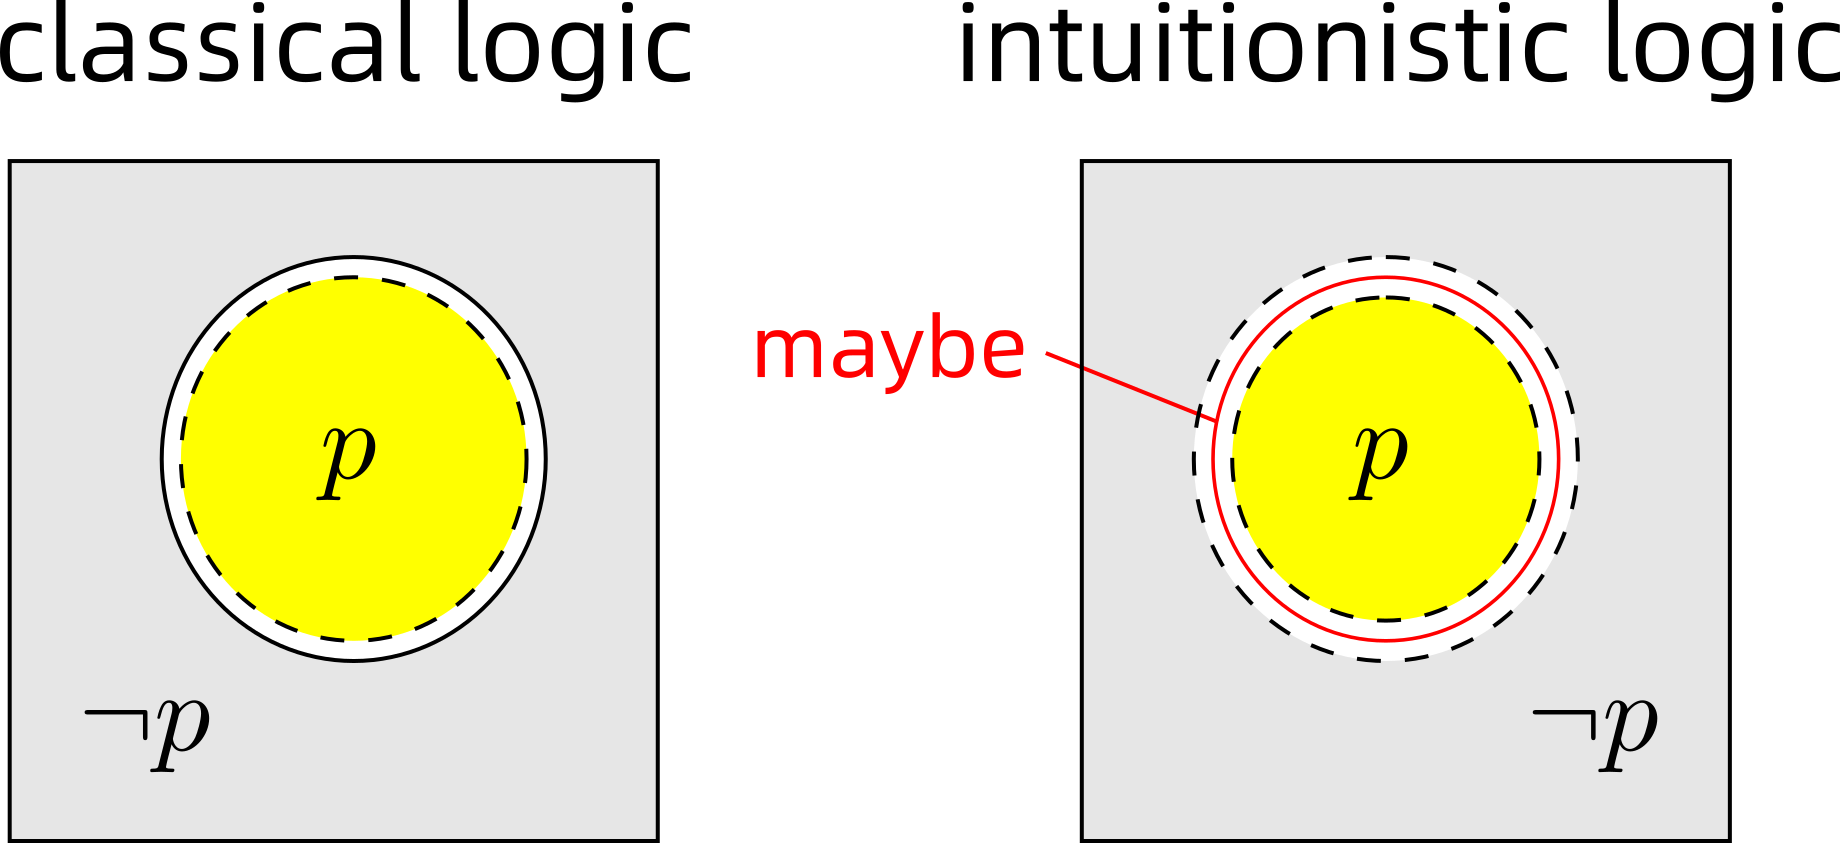
\includegraphics[scale=0.8]{topology-intuitionistic.png}}}
\end{equation}

\subsection{Higher-order logic}

Propositional logic 的意思是: 只有命题,但忽略任何 \textbf{命题内部} 的结构。 

假设 $p, q$ 是命题,命题逻辑的基本运算 就是 $p \wedge q, p \vee q, p \Rightarrow q, \neg p$.

First-order logic 的意思是: 容许 这样的方法 构成 命题:
\begin{equation}
\overbrace{\mbox{IsHuman}}^{\mbox{predicate}} ( \overbrace{\mbox{John}}^{\mbox{object}} ).
\end{equation}
Predicate 的意思是 \emp{谓词}; 谓词 是一些「有洞的命题」,它们被填入 objects 之后就变成完整的命题。 类似地可以有 \emp{多元}的 predicates,例如:
\begin{equation}
\mbox{Loves} (\mbox{John}, \mbox{Mary}).
\end{equation}
First-order 指的是: $\forall, \exists$ 这些 \emp{量词} 可以 \textbf{作用} 在 objects 的类别上,例如(Mary \textit{人见人爱}):
\begin{equation}
\forall x. \; \mbox{Loves}(x, \mbox{Mary})
\end{equation}
但 first-order logic 不容许 量词 作用在 predicates 的类别上,除非用 second-order logic.

一个 二阶逻辑的例子是「\textit{拿破仑 具有一个好将军应该具备的所有特质}」:
\begin{equation}
\forall p. \; p(\mbox{Good General}) \Rightarrow p(\mbox{Napoleon}).
\end{equation}
注意 $p$ 是在 predicates 的类别之上量化的。

\subsection{旧式 logic with type theory}

Type theory 的历史还可以追溯更早。 它起源於 Russell 为了解决 \emp{逻辑悖论},例如:「\textit{一个只帮自己不理发的人理发的理发师帮不帮自己理发?}」  这些 逻辑悖论 根源是在於: 定义一样东西的时候,中途 \textbf{指涉} 了这个东西本身。 这种不良的定义称作 \emp{impredicative}.  为了避免不良定义,每个东西出现之前必需「宣告」它的类型,这就是 type theory 原来的目的。 

在 Curry-Howard isomorphism 未被重视之前,有一种更简单地 用 type theory 定义 逻辑的方法。 在这种方法下,逻辑命题 $p, q, p \wedge q$ 等 \textbf{直接用} terms 定义,而不是像 Curry-Howard 那样,逻辑命题 = types,证明 = terms.

在这情况下 type theory 处理的是 (first- or higher-order) predicate logic 的方面。 这是说,例如:
\begin{equation}
\mbox{IsHuman} (\mbox{John})
\end{equation}
里面 IsHuman 是一个 函数 term,它输入一个 物体,输出它是不是「人」的真值 (truth value) $\in \Omega = \{ \top, \bot \}$.  因此 IsHuman 是一个 类型为 $\mbox{Obj} \rightarrow \Omega$ 的 term.

\cc{
这种做法没有容纳 Curry-Howard isomorphism 的馀地。 如果要做到后者,需要的是 Martin-L\"{o}f type theory....}{
This approach leaves no room to accommodate Curry-Howard isomorphism.  To do the latter, we would need Martin-L\"{o}f type theory....
}

\subsection{Martin-L\"{o}f type theory}

根据 Curry-Howard, 下面的 $A {\color{blue}\Rightarrow} B$ 是一个 逻辑命题,因而是 type: 
\begin{equation}
\vcenter{\hbox{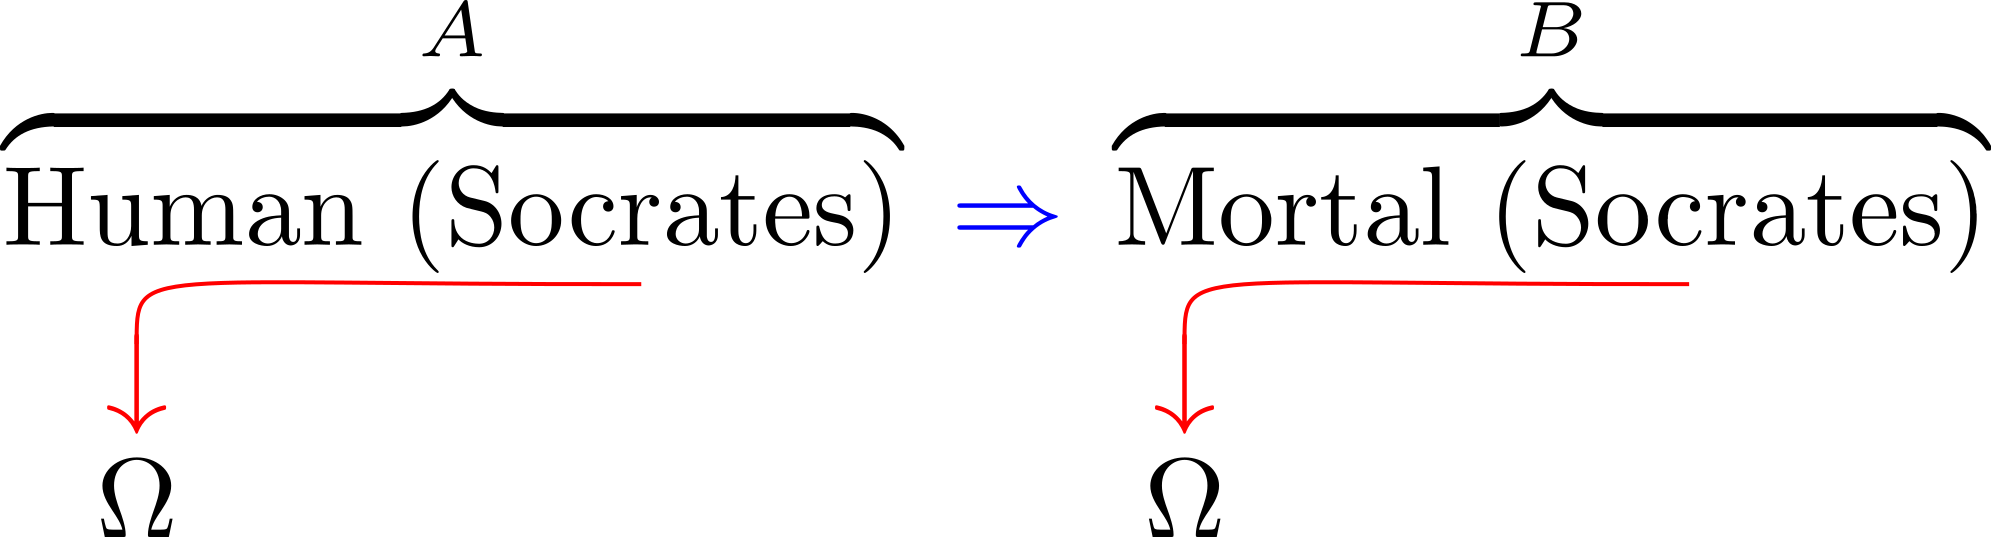
\includegraphics[scale=0.8]{why-Martin-Lof.png}}}
\end{equation}
但另方面,Human() 和 Mortal() 这两个 predicates 也需要借助 type theory 来构成命题,它们也是 types.  ${\color{red}\mbox{红色} \rightarrow}$ 和 ${\color{blue}\mbox{蓝色} \Rightarrow}$ 的两个层次 是完全不同的 两码子事,但因为 Curry-Howard 而被逼 挤在一起。 这就使得 type theory 好像「一心不能二用」。

在 ``simple'' type theory 里面可以 构造:
\begin{itemize}
	\item sum type $A + B$
	\item product type $A \times B$
	\item function type $A \rightarrow B$
\end{itemize}
分别对应於 直觉主义逻辑的 $\vee, \wedge, {\color{blue}\Rightarrow}$.  这些是在 \textbf{命题逻辑} 层面的,已经「用尽」了 type theory 的法宝。 

但 Human(Socrates) 也是由 Human() 和 Socrates 构成的命题,这构成的方法是用一个 arrow ${\color{red}\rightarrow}$,但已经没有 arrow 可用。 

Martin-L\"{o}f 提出的解决方案是 引入新的 type constructors:
\begin{itemize}
	\item \textbf{dependent} sum type $\Sigma$
	\item \textbf{dependent} product type $\Pi$
\end{itemize}

Dependent sum $\displaystyle \sum_A B$ 里面 $B$ 的类型 depends on $A$. 整个 family of A 的 + 的结果变成类似 product $A \times B$.

Dependent product $\displaystyle \prod_A B$ 里面 $B$ 的类型 depends on $A$. 整个 family of A 的 $\times$ 的结果变成类似 exponentiation $B^A$.

Dependent products can be used to define \textbf{predicates} such as Human() and Mortal().  They are of type $\displaystyle \mathrm{Obj} \rightarrow \Omega = \Omega^{\mathrm{Obj}} = \prod_{\mathrm{Obj}} \Omega$.  \footnote{Note that ``objects'' here mean logic objects, not objects in category theory.}

一个很漂亮的结果是: 如果用 $\sum_A B$ 和 $\prod_A B$ 定义 逻辑命题,则这些 types 如果被 inhabited 的话,分别对应於 $\exists A. B(A)$ 和 $\forall A. B(A)$. 这是因为: 如果 $A \times B$ inhabited,表示至少存在一个 $B(A)$; 而如果 $B^A$ inhabited,则存在一个函数,将任意的 $A$ send to $B$.

Per Martin-L\"{o}f (1942-) was the first logician to see the full importance of the connection between intuitionistic logic and type theory.

\subsection{Arithmetic-logic correspondence}

很多人都知道,经典逻辑中 $\wedge, \vee$ 对应於 \textbf{算术运算} $\times, +$(也可以看成是 fuzzy logic 的 $\min, \max$.) 其实这就是 George Boole 尝试将 \emp{逻辑} 变成 某种\emp{代数} 的原因。

较少人知道的是 $A \Rightarrow B$ 也对应於 $B^A$: \footnote{其中 $0^0$ 是「不确定式」,但根据 组合学 惯例可以定义为 1.}
\begin{equation}
\label{truth-table:material-implication}
\begin{tabular}{|c|c|c|c|}
	\hline 
	$A$ & $B$ & $A \Rightarrow B$ & $B^A$ \\ 
	\hline \hline 
	0 & 0 & 1 & $0^0 = 1$ \\
	\hline 
	0 & 1 & 1 & $1^0 = 1$ \\ 
	\hline 
	1 & 0 & 0 & $0^1 = 0$ \\ 
	\hline 
	1 & 1 & 1 & $1^1 = 1$ \\ 
	\hline 
\end{tabular} 
\end{equation}
这个惊奇的「巧合」似乎再一次证实 Curry-Howard correspondence 是正确的; 特别地,它意味 $\Rightarrow$ 应该看成是 \textbf{函数},即所谓 ``functional interpretation of logical deduction.'' 

更详细观察,table (\ref{truth-table:material-implication}) 里面 $A$ 和 $B$ 的 truth values 可以看成是它们的 types 有没有 \textbf{inhabitants}. Type $A$ 的 inhabitant 就是它的证明 $\square$,没有证明就是 $\emptyset$.  或者推广到:命题 $A$ 的真值 = $A$ 的 type 作为 集合 的 \textbf{cardinality}, $V(A) = |A|$.  这样看,$\Rightarrow$ 的真值 就是 $|B^A|$, 亦即是从 $\{\square\}$ 或 $\emptyset$ 到 $\{\square\}$ 或 $\emptyset$ 的 map, 而这个 map 只有在 $\emptyset \mapsto \{\square\}$ 的时候是空集(不可能)。

这个观察 可以推广到 fuzzy logic (\S\ref{sec:fuzzy-implication}) 和 strict implication $A \strictif B$ (\S\ref{sec:strict-implication}).

\section{Topos theory}

将 type theory 对应到 category theory,这工作是 Lambek 做的,於是完成了 Curry-Howard-Lambek 的「三位一体」。

想认识一个 \emp{范畴},最重要的是问: 它的 objects 是啥? 它的 morphisms 是啥? 

Lambek 给出的对应是:
\begin{itemize}
	\item types $\leftrightsquigarrow$ objects
	\item terms $\leftrightsquigarrow$ morphisms
\end{itemize}

\subsection{Classifying topos $\leftrightharpoons$ internal language}

We have the following transformations betweeen two formalisms:
\begin{equation}
\begin{tikzcd}[column sep = 20ex]
\boxed{\mbox{topos}} \; \mathcal{C}
\arrow[r, shift left, "\mbox{internal language}"]
& T \; \boxed{\mbox{type theory}}
\arrow[l, shift left, "\mbox{classifying topos}"]
\end{tikzcd}.
\end{equation}
In other words,
\begin{equation}
\mathcal{C} = \mathrm{Cl}(T), \quad T = \mathrm{Th}(\mathcal{C}).
\end{equation}

\subsection{$\forall$ and $\exists$ as adjunctions}

Let $\mbox{Forms}(\vec{x})$ denote the set of formulas with only the variables $\vec{x}$ free.

Then there is a trivial operation of adding an additional dummy variable $y$:
\begin{equation}
* : \mbox{Forms}(\vec{x}) \rightarrow \mbox{Forms}(\vec{x}, y)
\end{equation}
taking each formula $\phi(\vec{x})$ to itself.

It turns out that $\exists$ and $\forall$ are adjoints to the map $*$:
\begin{equation}
\exists \dashv * \dashv \forall
\end{equation}

\subsection{Sheaves and topos}

Some $\mathbf{Set}$-valued functors are \emp{representable}, ie, isomorphic to a hom-functor.

Functors $\mathcal{C} \rightarrow \mathbf{Set}$ are called \emp{pre-sheaves} on $\mathcal{C}$.

Sheaves capture ``indexing''.

\subsection{Yoneda lemma}

在一个范畴 $\mathcal{C}$ 里面,考虑 其中一个物体 $A$ 到其他物体的 morphism, $A \rightarrow \bullet$.  这可以说是,透过 $A$「看」其他物体的方法。

\textbf{例:} 在 $\mathbf{Set}$ 里面,$1 \rightarrow X$ 是用 终点物体 1「看」其他物体,看到的是集合的 \textbf{元素}。

\textbf{例:} 映射 $\mathbb{R} \rightarrow X$ 是 空间 $X$ 中的 \textbf{曲线},可以说 $\mathbb{R}$「看到」曲线。

\textbf{例:} 在 ordered set $(\mathbb{R}, \le)$ 里面 物体 $0 \rightarrow x$ 可以「看到」$x$ 是不是 \textbf{positive}.

类似地,可以考虑 对偶 的情况,$\bullet \rightarrow A$ 是其他物体怎样「看」$A$ 的方法。

\textbf{例:} 在 $\mathbf{Set}$ 里面,$X \rightarrow 2$ 是其他物体「看」2 的方式,得到的是 $X$ 的\textbf{子集}, $\powerset(X)$. 

\textbf{例:} 在 $\mathbf{Top}$ 里面,2 包含一个 open set 和一个 closed set,$X \rightarrow 2$ 得出的是 $X$ 的\textbf{开子集},$\mathrm{Opens}(X)$.



How sheaves gives rise to representables.

\subsection{Model theory, functorial semantics}

\subsection{Generalized elements and forcing}

一个 逻辑命题 $\phi$ 可以看成是由 某论域 $A \stackrel{\phi}{\rightarrow} \Omega$ 的函数,其中 $\Omega = \{ \top, \bot \}$.

也可以说:命题 $\phi(x)$ 是真的,其中 $x$ 是 $A$ 的\emp{元素}。 In category theory, we use the terminal object $1$ to ``pick out'' elements of $A$, as follows:
\begin{equation}
1 \stackrel{x}{\rightarrow} A \stackrel{\phi}{\rightarrow} \Omega.
\end{equation}
In $\mathbf{Set}$, 任意一个由 1 出发的函数 $x: 1 \rightarrow A$ 可以直接看成是 $A$ 的「元素」。

但如果我们用另一个 论域 $C$ 取代 1,换句话说:
\begin{equation}
C \stackrel{x}{\rightarrow} A \stackrel{\phi}{\rightarrow} \Omega.
\end{equation}
这样的 $x: C \rightarrow A$ 叫作 $A$ 的 \emp{generalized element}.

另一个术语是: $C$ \emp{forces} $\phi(x)$, notation $C \Vdash \phi(x)$. \\
或者说 $\phi(x)$ is true \emp{at stage} $C$ (这术语来自 possible-world semantics).

\subsection{Kripke-Joyal semantics}

An ``internal'' way to interpret type theory in a topos is where a formula $\phi$ in context $x_1: A_1, ... , x_n: A_n$ is interpreted as a subobject of $A_1 \times ... \times A_n$.  This has the disadvantage that the most pleasant illusion of ``elements'' is totally lost.

用 Kripke-Joyal semantics 可以挽回 generalized elements 的诠释方法。 

Generalized element 的意思是 $I \stackrel{a}{\rightarrow} A \stackrel{\phi}{\rightarrow} \Omega$ 记作 $a \Vdash \phi$.

\subsection{Cohen's (dis)proof of Continuum Hypothesis}

Continuum hypothesis (CH):
\begin{equation}
2^{\aleph_0} = \aleph_1
\end{equation}
这是说: 连续统 $[0,1]$ 的基数 $2^{\aleph_0}$ 紧接在 可数集合的基数 之后。

1878 年,Cantor 提出 CH \\
1900 年,Hilbert 列出 连续统假设 为「23问题」的第一个 \\
\tab Hilbert 给出了一个证明,但里面有 bug \\
1938 年,G\"{o}del 证明 ZF + CH is consistent,换句话说:ZF cannot disprove CH \\
1963 年,Paul Cohen 证明 ZF cannot prove CH \\
\tab 他用的方法叫 ``forcing''

\subsection{Kleene realizability}


\section{Intuitionistic logic}

G\"{o}del proposed an interpretation of intuitionistic logic using possible-world semantics.

In topos theory $A \Rightarrow B$ is adjoint (via the hom-product adjunction) to $A \vdash B$, which is ``okay'' because it is independent of which implication (material or strict) we are using.

\subsection{Heyting algebra}

In a topos $\mathbb{E}$, the subobject $\mathrm{Sub}_{\mathbb{E}}(A)$ is a \emp{poset} that admits \emp{Heyting implication}.  The Heyting implication $a \Rightarrow b$ exists for all elements $a, b, x$ such that:
\begin{equation}
x \le (a \Rightarrow b) \quad \mbox{iff} \quad (x \wedge a) \le b.
\end{equation}
Every Boolean algebra can be a Heyting algebra with the material implication defined as usual: $a \Rightarrow b \equiv \neg a \vee b$.

Heyting algebra is to intuitionistic logic what Boolean algebra is to classical logic.  But this may not jibe with the idea of ``strict implication''.

Under Kripke semantics, the Heyting arrow $\rightarrow$ can be defined by:
\begin{equation}
k \Vdash A \rightarrow B \quad \Leftrightarrow \quad \forall \ell \ge k \; (\ell \Vdash A \Rightarrow \ell \Vdash B)
\end{equation}

Whereas the ``fish-hook'' strict implication can be defined as:
\begin{equation}
A \strictif B \quad \equiv \quad \square (A \Rightarrow B) 
\end{equation}

The two can be regarded as equivalent via:
\begin{equation}
\begin{aligned}
k \Vdash \square (A \Rightarrow B) \quad \Leftrightarrow \quad & \forall \ell \ge k \; (\ell \Vdash (A \Rightarrow B)) \\
\quad \Leftrightarrow \quad & \forall \ell \ge k \; (\ell \Vdash A \Rightarrow \ell \Vdash B)
\end{aligned}
\end{equation}

\section{Modal logic}

Modalities are often conceived in terms of variation over some collection or \textbf{possible worlds}.

A modal operator (such as $\square$) in $\mathrm{Sheaf}(X)$ is a \emp{sheaf morphism} $\square: \Omega \rightarrow \Omega$ satisfying 3 conditions, for all $U \subseteq X$ and $p, q \in \Omega(U)$:
\begin{equation}
\begin{aligned}
& \mbox{a)} \quad p \le \square (p) \\
& \mbox{b)} \quad (\square ; \square) (p) \le \square (p) \\
& \mbox{c)} \quad \square (p \wedge q) = \square (p) \wedge \square (q)
\end{aligned}
\end{equation}

\subsection{Possible-world semantics}

Possible-world semantics is also called \emp{intensional semantics}, as opposed to \emp{extensional semantics} where truth values are directly assigned to propositions.  Does this idea jibe with the other definition of ``intension'', ie, as opposed to Leibniz extensionality and also related to intensional logic?

\subsection{Computer implementation of possible worlds}

要在电脑上实现 possible-world semantics 是不是很麻烦?

\subsection{Intensional vs extensional}

``Beethoven's 9th symphony'' and ``Beethoven's choral symphony'' has the same \emp{extension} but different \emp{intensions}.

\subsection{Intensional logic}

Possible-world semantics is also called \emp{intensional semantics}, as opposed to \emp{extensional semantics} where truth values are directly assigned to propositions.

Logic terms differ in intension if and only if it is \textbf{possible} for them to differ in extension.  Thus, \emp{intensional logic} interpret its terms using possible-world semantics.

\subsection{Strict implication}
\label{sec:strict-implication}

\subsubsection{The problem of ``material implication''}

Material implication 的意思是「实质蕴涵」,亦即是说 $A \Rightarrow B$ 等价於 $\neg A \vee B$,其真值表如下:

\begin{equation}
\label{eqn:implication-truth-table}
\begin{tabular}{|c|c|c|}
\hline 
$A$ & $B$ & $A \Rightarrow B$ \\ 
\hline \hline 
0 & 0 & 1 \\
\hline 
0 & 1 & 1 \\ 
\hline 
1 & 0 & 0 \\ 
\hline 
1 & 1 & 1 \\ 
\hline 
\end{tabular} 
\end{equation}

Material implication 的概念向来很有争议,例如,当前提是错误时,它永远是真的: 
\begin{equation}
\mbox{瑞士在非洲} \Rightarrow \mbox{猪会飞}
\end{equation}

\begin{center}
\rule{0.8\textwidth}{1pt}
\end{center}

透过观察 truth table 可以发现,它的每一列 其实代表一个 \emp{可能世界},这些 可能世界 是不会 同时发生的。 换句话说,material implication 和 strict implication 本来是一样的,只是前者将 可能世界 的语义 隐蔽到「幕后」。 

For strict implication to make sense, it is always necessary to invoke possible-world semantics.  A strict implication is always \emp{learned} from numerous examples from experience, in accord with the philosophical tradition of ``empiricism''.

Strict implication is equivalent to material implication over multiple instances.  The truth table of material implication agrees with the functional interpretation of implication.  

\section{Fuzzy logic}

首先是 implication 的问题,fuzzy implication 并不对应於 material implication in Boolean algebra.

另外有个问题就是要考察一下 fuzzy truth value 在各种情况下的正确性。 

例如假设 set 里面有 fuzzy proposition 的「证明」\\
又或者「人类」的集合是「有人类」这个命题的证明 \\
而,「数学家」作为「人类」的子集,等於命题「所有人都是数学家」的证明 \\
而这和 fuzzy value 是一致的

但为什么「John 是人」这个命题有点怪怪的? \\
如果它有 fuzzy value,应该是某集合的子集 \\
有些元素证明 John 是人,有些证明他不是人 \\
或者是 John 的\emp{属性}的集合? \\
而其中有些属性 imply 他是人? \\
或者有些属性 $\subseteq$ 人的属性?

还有这跟 ``Marilyn Monroe is sexy'' 是不是一致?
Marilyn 的所有属性集合,其中 imply sexy 的 subset \\
还是 sexy 的所有属性集合,其中 Marilyn 也有的?

Sexy(marilyn), Human(john), vs Human(Mathematicians).


What kind of mapping does this require?

\subsection{Fuzzy implication}
\label{sec:fuzzy-implication}

Implication 能不能 generalize 到 fuzzy logic 的情况?

\subsection{Fuzzy functions?}

What are fuzzy functions?

\section{Homotopy type theory (HoTT)}

HoTT 的中心思想是将 types 看成是某些 空间 (spaces),而这些空间可以被赋予 topological 特别是 homotopy 结构。 在 homotopy 而言,关键是 将 type $A$ 里面两个元素的 \textbf{相等} $id_A$ 看成是 homotopy 的 \textbf{path}.

\subsection{What is homotopy?}

\subsection{Univalence axiom}

在 HoTT 的 set 的层次,``='' 是一个 predicate, 根据我的理论可以看成是 fuzzy predicate.

如果我没理解错误,univalence axiom 的意思 似乎是将 = 的 fuzzy truth value「强制」成 binary.

\section*{References}
\cc{欢迎提问和讨论}{Questions, comments welcome} \smiley \\ \vspace*{0.4cm}
\printbibliography

\end{document} 
